
%% bare_conf.tex
%% V1.3
%% 2007/01/11
%% by Michael Shell
%% See:
%% http://www.michaelshell.org/
%% for current contact information.
%%
%% This is a skeleton file demonstrating the use of IEEEtran.cls
%% (requires IEEEtran.cls version 1.7 or later) with an IEEE conference paper.
%%
%% Support sites:
%% http://www.michaelshell.org/tex/ieeetran/
%% http://www.ctan.org/tex-archive/macros/latex/contrib/IEEEtran/
%% and
%% http://www.ieee.org/

%%*************************************************************************
%% Legal Notice:
%% This code is offered as-is without any warranty either expressed or
%% implied; without even the implied warranty of MERCHANTABILITY or
%% FITNESS FOR A PARTICULAR PURPOSE! 
%% User assumes all risk.
%% In no event shall IEEE or any contributor to this code be liable for
%% any damages or losses, including, but not limited to, incidental,
%% consequential, or any other damages, resulting from the use or misuse
%% of any information contained here.
%%
%% All comments are the opinions of their respective authors and are not
%% necessarily endorsed by the IEEE.
%%
%% This work is distributed under the LaTeX Project Public License (LPPL)
%% ( http://www.latex-project.org/ ) version 1.3, and may be freely used,
%% distributed and modified. A copy of the LPPL, version 1.3, is included
%% in the base LaTeX documentation of all distributions of LaTeX released
%% 2003/12/01 or later.
%% Retain all contribution notices and credits.
%% ** Modified files should be clearly indicated as such, including  **
%% ** renaming them and changing author support contact information. **
%%
%% File list of work: IEEEtran.cls, IEEEtran_HOWTO.pdf, bare_adv.tex,
%%                    bare_conf.tex, bare_jrnl.tex, bare_jrnl_compsoc.tex
%%*************************************************************************

% *** Authors should verify (and, if needed, correct) their LaTeX system  ***
% *** with the testflow diagnostic prior to trusting their LaTeX platform ***
% *** with production work. IEEE's font choices can trigger bugs that do  ***
% *** not appear when using other class files.                            ***
% The testflow support page is at:
% http://www.michaelshell.org/tex/testflow/



% Note that the a4paper option is mainly intended so that authors in
% countries using A4 can easily print to A4 and see how their papers will
% look in print - the typesetting of the document will not typically be
% affected with changes in paper size (but the bottom and side margins will).
% Use the testflow package mentioned above to verify correct handling of
% both paper sizes by the user's LaTeX system.
%
% Also note that the "draftcls" or "draftclsnofoot", not "draft", option
% should be used if it is desired that the figures are to be displayed in
% draft mode.
%
\documentclass[conference]{IEEEtran}
% Add the compsoc option for Computer Society conferences.
%
% If IEEEtran.cls has not been installed into the LaTeX system files,
% manually specify the path to it like:
% \documentclass[conference]{../sty/IEEEtran}


\usepackage{tikz}
\usetikzlibrary{decorations.pathmorphing}
\graphicspath{{./Figures/}}


% Some very useful LaTeX packages include:
% (uncomment the ones you want to load)


% *** MISC UTILITY PACKAGES ***
%
%\usepackage{ifpdf}
% Heiko Oberdiek's ifpdf.sty is very useful if you need conditional
% compilation based on whether the output is pdf or dvi.
% usage:
% \ifpdf
%   % pdf code
% \else
%   % dvi code
% \fi
% The latest version of ifpdf.sty can be obtained from:
% http://www.ctan.org/tex-archive/macros/latex/contrib/oberdiek/
% Also, note that IEEEtran.cls V1.7 and later provides a builtin
% \ifCLASSINFOpdf conditional that works the same way.
% When switching from latex to pdflatex and vice-versa, the compiler may
% have to be run twice to clear warning/error messages.






% *** CITATION PACKAGES ***
%
%\usepackage{cite}
% cite.sty was written by Donald Arseneau
% V1.6 and later of IEEEtran pre-defines the format of the cite.sty package
% \cite{} output to follow that of IEEE. Loading the cite package will
% result in citation numbers being automatically sorted and properly
% "compressed/ranged". e.g., [1], [9], [2], [7], [5], [6] without using
% cite.sty will become [1], [2], [5]--[7], [9] using cite.sty. cite.sty's
% \cite will automatically add leading space, if needed. Use cite.sty's
% noadjust option (cite.sty V3.8 and later) if you want to turn this off.
% cite.sty is already installed on most LaTeX systems. Be sure and use
% version 4.0 (2003-05-27) and later if using hyperref.sty. cite.sty does
% not currently provide for hyperlinked citations.
% The latest version can be obtained at:
% http://www.ctan.org/tex-archive/macros/latex/contrib/cite/
% The documentation is contained in the cite.sty file itself.






% *** GRAPHICS RELATED PACKAGES ***
%
\ifCLASSINFOpdf
%  \usepackage[pdftex]{graphicx}
  % declare the path(s) where your graphic files are
%  \graphicspath{{./Figures/}}
  % and their extensions so you won't have to specify these with
  % every instance of \includegraphics
%  \DeclareGraphicsExtensions{.pdf,.jpeg,.png}
\else
  % or other class option (dvipsone, dvipdf, if not using dvips). graphicx
  % will default to the driver specified in the system graphics.cfg if no
  % driver is specified.
 % \usepackage[dvips]{graphicx}
  % declare the path(s) where your graphic files are
%  \graphicspath{{./Figures/}}
  % and their extensions so you won't have to specify these with
  % every instance of \includegraphics
%  \DeclareGraphicsExtensions{.eps}
\fi
% graphicx was written by David Carlisle and Sebastian Rahtz. It is
% required if you want graphics, photos, etc. graphicx.sty is already
% installed on most LaTeX systems. The latest version and documentation can
% be obtained at: 
% http://www.ctan.org/tex-archive/macros/latex/required/graphics/
% Another good source of documentation is "Using Imported Graphics in
% LaTeX2e" by Keith Reckdahl which can be found as epslatex.ps or
% epslatex.pdf at: http://www.ctan.org/tex-archive/info/
%
% latex, and pdflatex in dvi mode, support graphics in encapsulated
% postscript (.eps) format. pdflatex in pdf mode supports graphics
% in .pdf, .jpeg, .png and .mps (metapost) formats. Users should ensure
% that all non-photo figures use a vector format (.eps, .pdf, .mps) and
% not a bitmapped formats (.jpeg, .png). IEEE frowns on bitmapped formats
% which can result in "jaggedy"/blurry rendering of lines and letters as
% well as large increases in file sizes.
%
% You can find documentation about the pdfTeX application at:
% http://www.tug.org/applications/pdftex





% *** MATH PACKAGES ***
%
%\usepackage[cmex10]{amsmath}
% A popular package from the American Mathematical Society that provides
% many useful and powerful commands for dealing with mathematics. If using
% it, be sure to load this package with the cmex10 option to ensure that
% only type 1 fonts will utilized at all point sizes. Without this option,
% it is possible that some math symbols, particularly those within
% footnotes, will be rendered in bitmap form which will result in a
% document that can not be IEEE Xplore compliant!
%
% Also, note that the amsmath package sets \interdisplaylinepenalty to 10000
% thus preventing page breaks from occurring within multiline equations. Use:
%\interdisplaylinepenalty=2500
% after loading amsmath to restore such page breaks as IEEEtran.cls normally
% does. amsmath.sty is already installed on most LaTeX systems. The latest
% version and documentation can be obtained at:
% http://www.ctan.org/tex-archive/macros/latex/required/amslatex/math/





% *** SPECIALIZED LIST PACKAGES ***
%
%\usepackage{algorithmic}
% algorithmic.sty was written by Peter Williams and Rogerio Brito.
% This package provides an algorithmic environment fo describing algorithms.
% You can use the algorithmic environment in-text or within a figure
% environment to provide for a floating algorithm. Do NOT use the algorithm
% floating environment provided by algorithm.sty (by the same authors) or
% algorithm2e.sty (by Christophe Fiorio) as IEEE does not use dedicated
% algorithm float types and packages that provide these will not provide
% correct IEEE style captions. The latest version and documentation of
% algorithmic.sty can be obtained at:
% http://www.ctan.org/tex-archive/macros/latex/contrib/algorithms/
% There is also a support site at:
% http://algorithms.berlios.de/index.html
% Also of interest may be the (relatively newer and more customizable)
% algorithmicx.sty package by Szasz Janos:
% http://www.ctan.org/tex-archive/macros/latex/contrib/algorithmicx/




% *** ALIGNMENT PACKAGES ***
%
%\usepackage{array}
% Frank Mittelbach's and David Carlisle's array.sty patches and improves
% the standard LaTeX2e array and tabular environments to provide better
% appearance and additional user controls. As the default LaTeX2e table
% generation code is lacking to the point of almost being broken with
% respect to the quality of the end results, all users are strongly
% advised to use an enhanced (at the very least that provided by array.sty)
% set of table tools. array.sty is already installed on most systems. The
% latest version and documentation can be obtained at:
% http://www.ctan.org/tex-archive/macros/latex/required/tools/


%\usepackage{mdwmath}
%\usepackage{mdwtab}
% Also highly recommended is Mark Wooding's extremely powerful MDW tools,
% especially mdwmath.sty and mdwtab.sty which are used to format equations
% and tables, respectively. The MDWtools set is already installed on most
% LaTeX systems. The lastest version and documentation is available at:
% http://www.ctan.org/tex-archive/macros/latex/contrib/mdwtools/


% IEEEtran contains the IEEEeqnarray family of commands that can be used to
% generate multiline equations as well as matrices, tables, etc., of high
% quality.


%\usepackage{eqparbox}
% Also of notable interest is Scott Pakin's eqparbox package for creating
% (automatically sized) equal width boxes - aka "natural width parboxes".
% Available at:
% http://www.ctan.org/tex-archive/macros/latex/contrib/eqparbox/





% *** SUBFIGURE PACKAGES ***
%\usepackage[tight,footnotesize]{subfigure}
% subfigure.sty was written by Steven Douglas Cochran. This package makes it
% easy to put subfigures in your figures. e.g., "Figure 1a and 1b". For IEEE
% work, it is a good idea to load it with the tight package option to reduce
% the amount of white space around the subfigures. subfigure.sty is already
% installed on most LaTeX systems. The latest version and documentation can
% be obtained at:
% http://www.ctan.org/tex-archive/obsolete/macros/latex/contrib/subfigure/
% subfigure.sty has been superceeded by subfig.sty.



%\usepackage[caption=false]{caption}
%\usepackage[font=footnotesize]{subfig}
% subfig.sty, also written by Steven Douglas Cochran, is the modern
% replacement for subfigure.sty. However, subfig.sty requires and
% automatically loads Axel Sommerfeldt's caption.sty which will override
% IEEEtran.cls handling of captions and this will result in nonIEEE style
% figure/table captions. To prevent this problem, be sure and preload
% caption.sty with its "caption=false" package option. This is will preserve
% IEEEtran.cls handing of captions. Version 1.3 (2005/06/28) and later 
% (recommended due to many improvements over 1.2) of subfig.sty supports
% the caption=false option directly:
%\usepackage[caption=false,font=footnotesize]{subfig}
%
% The latest version and documentation can be obtained at:
% http://www.ctan.org/tex-archive/macros/latex/contrib/subfig/
% The latest version and documentation of caption.sty can be obtained at:
% http://www.ctan.org/tex-archive/macros/latex/contrib/caption/




% *** FLOAT PACKAGES ***
%
%\usepackage{fixltx2e}
% fixltx2e, the successor to the earlier fix2col.sty, was written by
% Frank Mittelbach and David Carlisle. This package corrects a few problems
% in the LaTeX2e kernel, the most notable of which is that in current
% LaTeX2e releases, the ordering of single and double column floats is not
% guaranteed to be preserved. Thus, an unpatched LaTeX2e can allow a
% single column figure to be placed prior to an earlier double column
% figure. The latest version and documentation can be found at:
% http://www.ctan.org/tex-archive/macros/latex/base/



%\usepackage{stfloats}
% stfloats.sty was written by Sigitas Tolusis. This package gives LaTeX2e
% the ability to do double column floats at the bottom of the page as well
% as the top. (e.g., "\begin{figure*}[!b]" is not normally possible in
% LaTeX2e). It also provides a command:
%\fnbelowfloat
% to enable the placement of footnotes below bottom floats (the standard
% LaTeX2e kernel puts them above bottom floats). This is an invasive package
% which rewrites many portions of the LaTeX2e float routines. It may not work
% with other packages that modify the LaTeX2e float routines. The latest
% version and documentation can be obtained at:
% http://www.ctan.org/tex-archive/macros/latex/contrib/sttools/
% Documentation is contained in the stfloats.sty comments as well as in the
% presfull.pdf file. Do not use the stfloats baselinefloat ability as IEEE
% does not allow \baselineskip to stretch. Authors submitting work to the
% IEEE should note that IEEE rarely uses double column equations and
% that authors should try to avoid such use. Do not be tempted to use the
% cuted.sty or midfloat.sty packages (also by Sigitas Tolusis) as IEEE does
% not format its papers in such ways.





% *** PDF, URL AND HYPERLINK PACKAGES ***
%
%\usepackage{url}
% url.sty was written by Donald Arseneau. It provides better support for
% handling and breaking URLs. url.sty is already installed on most LaTeX
% systems. The latest version can be obtained at:
% http://www.ctan.org/tex-archive/macros/latex/contrib/misc/
% Read the url.sty source comments for usage information. Basically,
% \url{my_url_here}.





% *** Do not adjust lengths that control margins, column widths, etc. ***
% *** Do not use packages that alter fonts (such as pslatex).         ***
% There should be no need to do such things with IEEEtran.cls V1.6 and later.
% (Unless specifically asked to do so by the journal or conference you plan
% to submit to, of course. )


% correct bad hyphenation here
\hyphenation{op-tical net-works semi-conduc-tor}

\usepackage{url}
\usepackage{booktabs,multirow,multicol}
\usepackage{cite}
\usepackage[latin1]{inputenc}
%\usepackage{subfigure}
\usepackage{caption}
\usepackage{subcaption}



\begin{document}
%
% paper title
% can use linebreaks \\ within to get better formatting as desired
\title{Hierarchical Classification of Gene Ontology-based Protein Functions with Neural Networks}
%\title{Predicting Gene Ontology-based Protein Functions with Neural Networks}
%\title{Hierarchical Multi-label Classification of Gene Ontology Terms with Neural Networks}


% author names and affiliations
% use a multiple column layout for up to three different
% affiliations
\author{\IEEEauthorblockN{Ricardo Cerri}
\IEEEauthorblockA{Department of Computing\\
Federal University of São Carlos\\
Rodovia Washington Luís, km 235\\
São Carlos, SP, Brazil\\
Email: cerrirc@gmail.com}
\and
\IEEEauthorblockN{Rodrigo C. Barros}
\IEEEauthorblockA{Faculdade de Informática\\
Pontifícia Universidade Católica do RS\\
Av. Ipiranga, 6681\\ Porto Alegre, RS, Brazil\\
Email: rodrigo.barros@pucrs.br}
\and
\IEEEauthorblockN{André C. P. L. F. de Carvalho}
\IEEEauthorblockA{Departamento de Ciência da Computação\\
Universidade de São Paulo\\
Av. Trabalhador Sao-Carlense, 400\\
São Carlos, SP, Brazil\\
Email: andre@icmc.usp.br}}

% conference papers do not typically use \thanks and this command
% is locked out in conference mode. If really needed, such as for
% the acknowledgment of grants, issue a \IEEEoverridecommandlockouts
% after \documentclass

% for over three affiliations, or if they all won't fit within the width
% of the page, use this alternative format:
% 
%\author{\IEEEauthorblockN{Michael Shell\IEEEauthorrefmark{1},
%Homer Simpson\IEEEauthorrefmark{2},
%James Kirk\IEEEauthorrefmark{3}, 
%Montgomery Scott\IEEEauthorrefmark{3} and
%Eldon Tyrell\IEEEauthorrefmark{4}}
%\IEEEauthorblockA{\IEEEauthorrefmark{1}School of Electrical and Computer Engineering\\
%Georgia Institute of Technology,
%Atlanta, Georgia 30332--0250\\ Email: see http://www.michaelshell.org/contact.html}
%\IEEEauthorblockA{\IEEEauthorrefmark{2}Twentieth Century Fox, Springfield, USA\\
%Email: homer@thesimpsons.com}
%\IEEEauthorblockA{\IEEEauthorrefmark{3}Starfleet Academy, San Francisco, California 96678-2391\\
%Telephone: (800) 555--1212, Fax: (888) 555--1212}
%\IEEEauthorblockA{\IEEEauthorrefmark{4}Tyrell Inc., 123 Replicant Street, Los Angeles, California 90210--4321}}




% use for special paper notices
%\IEEEspecialpapernotice{(Invited Paper)}




% make the title area
\maketitle


\begin{abstract}
%\boldmath
Hierarchical Multi-label Classification (HMC) is a classification problem where classes are organized in a hierarchical taxonomy, and instances can be simultaneously classified in more than one path of this hierarchy. In this paper, we investigate the HMC problem of classifying proteins in functions organized according to the Gene Ontology hierarchical taxonomy. This is a very complex task, since the Gene Ontology hierarchy is organized as a Directed Acyclic Graph with thousands of classes represented as terms of the hierarchy. We propose a neural network-based method to incorporate label-dependency during learning. The experimental results showed that the proposed method achieved competitive results when compared to the state-of-the-art methods in the literature.
\end{abstract}
% IEEEtran.cls defaults to using nonbold math in the Abstract.
% This preserves the distinction between vectors and scalars. However,
% if the conference you are submitting to favors bold math in the abstract,
% then you can use LaTeX's standard command \boldmath at the very start
% of the abstract to achieve this. Many IEEE journals/conferences frown on
% math in the abstract anyway.

% no keywords




% For peer review papers, you can put extra information on the cover
% page as needed:
% \ifCLASSOPTIONpeerreview
% \begin{center} \bfseries EDICS Category: 3-BBND \end{center}
% \fi
%
% For peerreview papers, this IEEEtran command inserts a page break and
% creates the second title. It will be ignored for other modes.
\IEEEpeerreviewmaketitle

\section{Introduction}

In traditional classification problems, an instance $\mathbf{x}_i \in X$ can be classified in only one class $c_j \in C$. Nonetheless, there are more complex classification tasks, where an instance can be simultaneously classified into a set of classes $C_j \in C$. One of this tasks is called Hierarchical Multi-Label Classification (HMC), in which an instance can be classified into a set of classes that are previously organized as a hierarchy, with subclasses and superclasses. In this hierarchy, superclass relationships are represented by a partial order $\prec_h$, \emph{i.e.}, for all $c_1, c_2 \in C, c_1 \prec_h c_2$ if and only if $c_1$ is a superclass of $c_2$.

Protein Function Prediction (PFP) is one of the most important applications related to HMC, because proteins perform many important functions within an organism. Proteins are related to biochemical reactions, cell signaling, structural, and mechanical functions~\cite{Costa2008}, to name a few. Given that protein functions are hierarchically related, PFP can be considered a typical HMC problem.

In this work, we make use of the Gene Ontology (GO) hierarchy to investigate the PFP problem. In the GO, classes are organized as a Directed Acyclic Graph (DAG) hierarchy of terms, in which each term corresponds to a protein function. The hierarchy comprises three ontologies covering different domains, each one with thousands of classes: {\it cellular components}, {\it biological processes}, and {\it molecular functions}~\cite{Ashburner2000}. Figure~\ref{fig:GO} illustrates a small part of the GO taxonomy.

\begin{figure*}[ht]
    \centering
    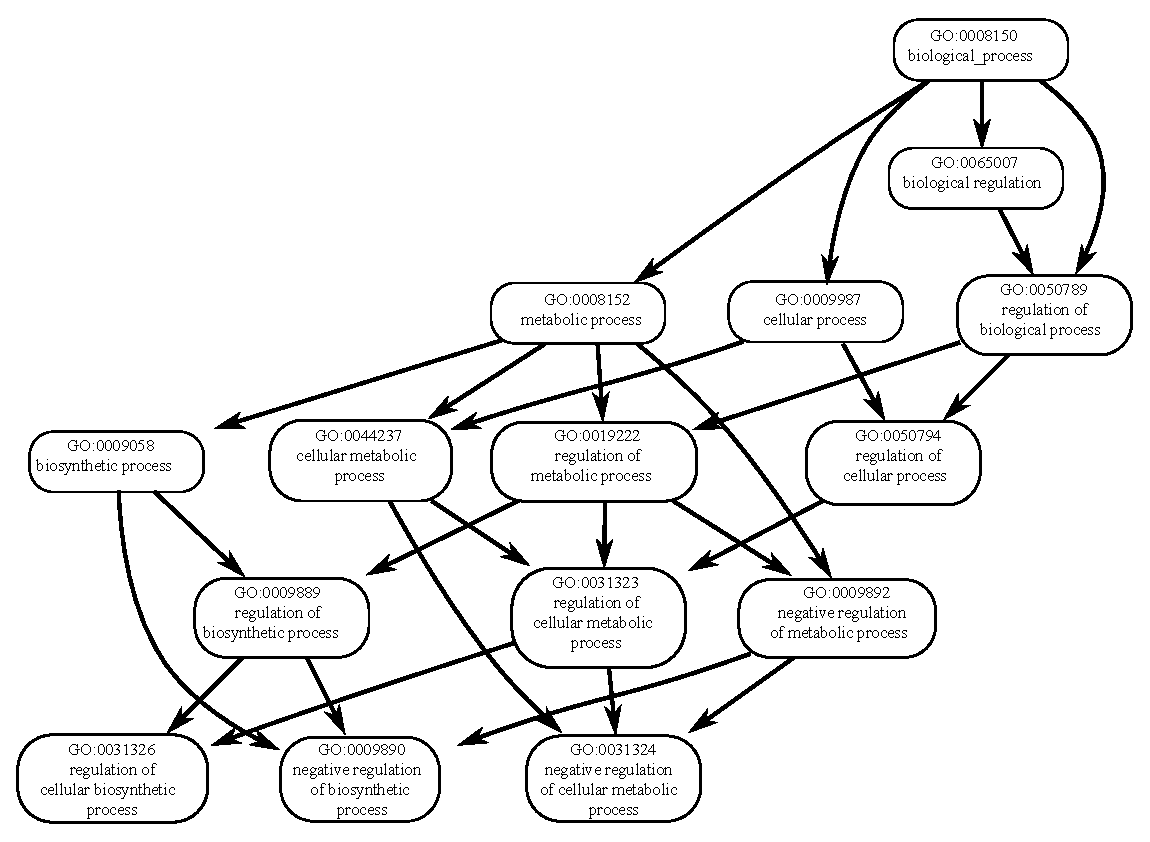
\includegraphics[scale=0.7]{GO-Taxonomy}
    \caption{Part of the Gene Ontology Hierarchical Taxonomy. (Adapted from Ashburner et. al. \cite{Ashburner2000})}
    \label{fig:GO}
\end{figure*}

The PFP task using the GO taxonomy is a very challenging problem. As we traverse the hierarchy down to the leaves, making accurate predictions becomes more difficult since terms have fewer and fewer positive instances. In addition, instances can be classified simultaneously into two or more paths of the hierarchy, and a term can have more than one parent node. We work with the ``is-a'' relation, which forms the basic structure of the GO. Thus, A is a B means that term A is a subtype of term B. Also, classifying an instance into class $c_j$ means that we are classifying it into all superclasses of class $c_j$. This is the multiple inheritance interpretation, which is the correct interpretation when working with the GO~\cite{Ashburner2000}.

%Two approaches have been used to solve HMC problems: local and global. In the local approach, conventional classification algorithms, such as decision tree induction algorithms or support vector machines, are trained to produce a hierarchy of classifiers. A classification for a new instance is then obtained combining the predictions provided by the individual classifiers~\cite{Costa2007}. In this approach, local information about the class hierarchy is used during the induction of each base classifier. According to \cite{Silla2010}, this local information can be used in different ways, depending on how the local classifiers are induced. The three main strategies for using local information are: one Local Classifier per Node (LCN), one Local Classifier per Parent Node (LCPN), and one Local Classifier per Level (LCL). The LCN strategy trains one binary classifier for each class of the hierarchy \cite{Valentini2009}. The LCPN strategy  trains, for each internal class, a multi-class classifier to distinguish between its subclasses \cite{Svetlana2004}, and the LCL strategy trains one multi-class classifier for each hierarchical level, where each classifier is responsible for the prediction in its associated level~\cite{Cerri2013}.

%Different from the local approach, the global approach induces a single classifier using all classes of the hierarchy at once. After the training process, the classification of a new instance by the induced classifier occurs in just one step \cite{Vens2008}. As global methods induce a single classifier to consider the specificities of the classification problem, they usually do not make use of conventional classification algorithms, unless these are adapted to consider the hierarchy of classes~\cite{Otero2010}.

The novel contributions of this paper are as follows. First, we propose a method called {\bf H}ierarchical {\bf M}ulti-Label {\bf C}lassification with {\bf L}ocal {\bf M}ulti-{\bf L}ayer {\bf P}erceptron (HMC-LMLP), which associates an MLP to each level of the hierarchy, in which each MLP is responsible for the predictions in its associated level. A very preliminary version of HMC-LMLP has been reported in \cite{Cerri2013}. Differently from the version in \cite{Cerri2013}, we employ the labels of the training instances as part of the input to train each MLP. Therefore, when training an MLP for level $l$, the feature vector of an instance is augmented with its classes for the level $l-1$. With this modification, we try to enforce the label dependencies between classes to be taken into account. We also propose a second version which ignores the labels associated with the classes to augment the feature vectors of the instances. This can be considered as a baseline version that allows us to examine whether the use of the labels to augment the feature vectors results in performance improvement.

Second, we employ the Local Classifier per Level (LCL)~\cite{Silla2010} strategy to make use of local information within each level of the hierarchy. By using one classifier per level we do not decompose the classification problem into a large number of sub-problems. The use of many classifiers per level may result in the application of over-specific local information, loss of important information, and loss of label dependency during training~\cite{Silla2010}. Finally, we present an analysis of the application of the LCL strategy to DAG-structured class hierarchies, adapting the DAG structure datasets in order to use them in the experiments. %Verifying the performance of the LCL strategy in very deep hierarchies with thousands of classes and class relationships is of great interest to researchers working with HMC problems.

%by using the LCL strategy, we intend to avoid deficiencies of both local and global methods. Unlike the global approach, HMC-LMLP is able to use local information which can be very useful to explore different data patterns in distinct hierarchical levels. Also, differently from the LCN and LCPN strategies, HMC-LMLP does not decompose the classification problem into a large number of sub-problems. The use of many classifiers per level may result in the application of over-specific local information, loss of important information, and loss of label dependency during training~\cite{Silla2010}. 

The remainder of this paper is organized as follows. Section~\ref{sec:relatedWork} presents related work regarding HMC for PFP. The proposed HMC-LMLP method is detailed in Section~\ref{sec:HMC-LMLP}, whereas a thorough empirical analysis is carried out in Section~\ref{sec:experiments}. A deeper discussion on the results is performed in Section~\ref{sec:discussion}, and the final considerations and future research directions are presented in Section~\ref{sec:conclusion}.


\section{Related Work}\label{sec:relatedWork}

This section discusses recent HMC methods reported in the literature that employ machine learning for protein and gene function prediction.

In Vens et al. \cite{Vens2008}, three methods based on the concept of Predictive Clustering Trees (PCT) were investigated. The authors proposed the Clus-HMC method that induces a single decision tree to cope with the entire classification problem. They compared its performance with two methods. The first one, Clus-SC, induces an independent decision tree for each class, ignoring the relationships between classes. The second one, Clus-HSC, explores the hierarchical relationships between the classes to induce a decision tree for each class. %Still based on PCT, the study of Schietgat et al. \cite{Schietgat2010} used an ensemble technique to combine the decision trees induced by Clus-HMC.

Alves et al. \cite{Alves2010} proposed a global method using Artificial Immune Systems (AIS) for the generation of HMC rules. The method is divided into two basic procedures: Sequential Covering (SC) and Rule Evolution (RE). The SC procedure iteratively calls the RE procedure until every (or almost every) training instance (antigens) is covered by the discovered rules. The RE procedure evolves classification rules (antibodies) that are employed to classify the instances. The best antibody is added to the set of discovered rules.

%An ensemble of LCN-based classifiers was proposed by Valentini \cite{Valentini2009}. In this method, each trained classifier estimates the local probability at which a given instance belongs to a given class. A combination phase estimates the global consensual probability. In \cite{ValentiniRe2009} and \cite{Valentini2011}, the authors modified this method to modulate the relationship between the prediction of a class and the prediction of its descendants.

In the work of Otero et al. \cite{Otero2010}, the authors proposed a method using Ant Colony Optimization (ACO). The method discovers classification rules, where an ACO algorithm is employed to optimize the antecedents of the rules. A sequential covering procedure is applied to create classification rules that cover most of the training instances. The method is initialized with an empty set of rules, and a new rule is added to the set while the number of instances not covered by any rule is higher than a given threshold. 

Cesa-Bianchi and Valentini \cite{Cesa-Bianchi2011} investigated the synergy between different LCN-based strategies related to gene function prediction task in FunCat annotated genes. They integrated kernel-based data fusion tools and ensemble algorithms with cost sensitive HMC methods \cite{Cesa-Bianchi2010,Valentini2011}. The authors defined synergy as the improvement in the prediction accuracy, considering any evaluation measure, due to the use of concurrent learning strategies. The synergy is detected when the combined action of two strategies achieves better correct classification rates than the average of the correct classification of the two strategies used separately~\cite{Cesa-Bianchi2011}.

Kordmahalleh et. al.~\cite{Kordmahalleh2013} proposed CAM-HMC, an evolutionary algorithm which applies evolutionary crowding niching and adaptive mutation to evolve antecedentes of HMC rules. During the evolutionary process, the authors defined a new distance measure $d$ for the competition between parents $p$ and offspring $c$. If $|d(p_1,c_1) + d(p_2,c_2)| \leq |d(p_1,c_2) + d(p_2,c_1)|$ the competition is between $(p_1,c_1)$ and $(p_2,c_2)$. Otherwise, the competition is between $(p_1,c_2)$ and $(p_2,c_1)$. The individuals with highest fitness are kept in the population. %The method also applies an adaptive range mutation introduced by Austin~\cite{Austin2002} to ensure uniform exploration of the search~space.

The work of Stojanova et. al.~\cite{Stojanova2013} proposed a method which considers autocorrelation in HMC, \emph{i.e.}, the statistical relationships between the same variable on different but related instances. The method is called Network Hierarchical Multi-label Classification (NHMC), and builds a generalized form of decision trees using the PCT framework, just like Clus-HMC. During training, NHMC uses both the features of the instances, and the autocorrelations between instances. The autocorrelations were modeled as a network, which is exploited by the method during the learning phase.

A genetic algorithm was proposed by Cerri et. al.~\cite{Cerri2014}. The method, called HMC-GA, evolves the antecedents of HMC rules, containing both propositional and relational tests. The consequents of the rules are deterministically obtained based on the classes of the training instances covered by the antecedents. Each generated rule is able to classify instances into two or more paths of the GO taxonomy.

Bi and Kwok~\cite{Bi2014} proposed a method which uses the Mandatory Leaf Node Prediction strategy (MLNP)~\cite{Silla2010}. The method uses hierarchy information, and the problem is formulated as finding the multiple labels with the largest posterior probability over all the labels. The authors extended the nested approximation property~\cite{Baraniuk2010} to deal with HMC problems structured as DAG, and solved the problem using a greedy algorithm (MAS).

In this paper, we make use of four methods reviewed in this section: Clus-HMC (which is considered to be the state-of-the-art method in the literature), Clus-HSC and Clus-SC. We also make use of the Ant Colony Optimization-based method {\it hm}Ant-Miner, which obtained competitive results with Clus-HMC. We chose these methods because they were all applied to the same datasets used in our experiments. In addition, they produce the same type of output provided by our proposed approach, and they have their code available for downloading, providing a fair base for comparison.
\section{HMC-LMLP}\label{sec:HMC-LMLP}

HMC-LMLP divides the learning process into a number of steps, combining MLPs individually trained for each level of the class hierarchy. The rationale is that each MLP learns something different from each other, breaking down the complex learning process into simpler~processes.

In HMC-LMLP, the MLPs are responsible for extracting local information from the instances at each level, which we believe to be useful in the classification of unlabeled instances. Our hypothesis is that different patterns can be extracted from instances in different hierarchical levels. Note that, whereas many different classifiers could be employed, we decided to choose neural networks because of the simplicity in associating a class per output neuron. Therefore, generating a multi-label prediction for a given instance is done in a straightforward fashion.

In this section, we present the proposed HMC-LMLP versions, called HMC-LMLP-Comp. These versions employ, at each level, the true labels of the instances from the previous level to augment the feature vectors. The second version is named HMC-LMLP-NoComp, since it only uses the original feature vectors to train an MLP at each level. For simplicity, all networks used in this study have a single hidden layer.

\subsection{HMC-LMLP-Comp}

Figure~\ref{fig:HMC-LMLP-Comp} illustrates the architecture of HMC-LMLP-Comp and its training process for a hierarchy with three levels. In this figure, $T_l$ are the true class labels associated to the instances at the level $l$; ${\bf X}^l$ represents the instances assigned to classes from the level $l$; $h_l$ and $O_l$ are, respectively, the hidden layer and output layer of the MLP network associated with level $l$. The matrices ${\bf W}_{1l}$ and ${\bf W}_{2l}$ represent, respectively, the weights connecting the input attributes and the neurons in the hidden layer, and the neurons in the hidden and output layers of the MLP associated with~level~$l$.

The neural network associated with the first level is trained with all training instances (${\bf X}^1$), since all instances are assigned to the classes from the first hierarchical level. At the second level, the MLP input is now the training instances that are assigned to the classes belonging to level 2 (${\bf X}^2$), combined with their true assigned classes in the first level. The advantage of using the augmented feature vector for training each MLP is the incorporation of label dependency. This process is repeated for each level of the hierarchy.

%\begin{figure*}[htbp]
%       \centering
%       
\includegraphics[scale=0.45]{HMC-LMLP-True}
%       \caption{Example of the HMC-LMLP-Comp architecture. (a) Training an MLP at the first level; (b) Using the true classes of the instances in level 1 to augment the feature vector of the instances used to train the MLP at the second level; (c) Using the true classes of the instances in level 2 to  augment the feature vector of the instances used to train the MLP at the third level.}
%       \label{fig:HMC-LMLP-True}
%\end{figure*}

As can be observed in the figure, the training process of HMC-LMLP-Comp, for each hierarchical level, can be performed in parallel, which can speed up the training process.

\subsection{HMC-LMLP-NoComp}

In HMC-LMLP-NoComp, an individual MLP is trained for each hierarchical level without employing the class labels to augment the feature vectors of the training instances. Figure~\ref{fig:HMC-LMLP-NoComp} illustrates the HMC-LMLP-NoLabels architecture and the training process. Similarly to HMC-LMLP-Comp, the training process in each level can be performed in parallel.

%\begin{figure*}[htbp]
%       \centering
%       
\includegraphics[scale=0.45]{HMC-LMLP-NoLabels}
%       \caption{Example of the HMC-LMLP-NoLabels architecture. (a) Training an MLP at the first level; (b) Training an MLP at the second level; (c) Training an MLP at the third level.}
%       \label{fig:HMC-LMLP-NoComp}
%\end{figure*}

\begin{figure*}[!htpb]
        \begin{subfigure}[b]{0.48\textwidth}
                \centering
                
\includegraphics[scale=0.5]{HMC-LMLP-True}
                \caption{Example of the HMC-LMLP-Comp architecture. (1) Training an MLP at the first level; (2) Using the true classes of the training instances in level 1 to augment the feature vector of the instances responsible for training the MLP at the second level; (3) Using the true classes of the training instances in level 2 to augment the feature vectors which are used for training the MLP at the third level.}
                \label{fig:HMC-LMLP-Comp}
        \end{subfigure}
		\hspace{10pt}
        \begin{subfigure}[b]{0.48\textwidth}
                \centering
                
\includegraphics[scale=0.5]{HMC-LMLP-NoLabels}
                \caption{Example of the HMC-LMLP-NoComp architecture. (1) Training an MLP at the first level; (2) Training an MLP at the second level; (3) Training an MLP at the third level.}
                \label{fig:HMC-LMLP-NoComp}
        \end{subfigure}
        \caption{Example of HMC-LMLP-Comp and HMC-LMLP-NoComp architectures for a three-level hierarchy.}
        \label{fig:HMC-LMLP}
\end{figure*}

\subsection{Obtaining final predictions}

In the test phase of HMC-LMLP-Comp (i.e., when predicting a test instance), the true labels are not available. Thus, a top-down strategy is employed, in which the feature vectors that are used for training the MLP at level $l$ are augmented with the output provided by the MLP in the level $l-1$. Due to this network dependency, the testing process of HMC-LMLP-Comp cannot be performed in parallel. Instead, the predictions for each level have to be obtained sequentially. In HMC-LMLP-NoComp, the testing phase is performed by feeding all instances into all MLPs at every level. Each MLP then provides independent predictions for the instances at each level. Thus, both training and testing phases, for each level, can be performed in parallel.

%The test instance is fed to the first MLP  (first level), and predictions for this level are obtained. As the true labels are not available in the test phase, the feature vectors of the instances used to train the MLP at the second level are complemented with the output provided by the MLP associated to the first level. This augmented feature vector is then used as input to the MLP associated with the second level, whose prediction values will, once again, complement the input for the MLP at the third level. This procedure is repeated until the last MLP network, associated with the last level, is reached. Recall that the augmentation of feature vectors is not incremental, \emph{i.e.}, the feature vector of an instance being fed into an MLP associated with level $l$ is only complemented by the output from the MLP associated with level~$l-1$.

%Because we use, in each level $l$, the predictions provided in level $l-1$, the testing process of HMC-LMLP-Comp cannot be performed in parallel. Instead, the predictions for each level have to be obtained sequentially. In HMC-LMLP-NoComp, the testing phase is performed feeding all instances into all MLPs at every level. Each MLP then gives independent predictions for the instances at each level. Thus, both training and testing phases, for each level, can be performed in parallel.

After obtaining the MLP outputs values, they are tested against thresholds in order to define the predictions for each level. If the output of a given neuron $j$ is greater than or equal to a given threshold, the instance that is being classified is assigned to class $c_j$. The final classification from HMC-LMLP is given by a binary vector ${\bf{v}}$ of size $|C|$, where $C$ is the set of all classes in the hierarchy. If the output value of neuron $j$ is greater than or equal to a given threshold, the value 1 is assigned to position ${\bf v}_j$. Otherwise, the position is set to 0. Since the activation function that is used in the neurons is the logistic sigmoid function, the output values range between 0 and 1. Thus, we can make use of threshold values also ranging from 0 to 1. The larger the threshold, the lower the number of predicted classes. Conversely, the lower the threshold, the larger the number of predicted~classes.

After testing the predictions against the thresholds, there could be classification inconsistencies, \emph{i.e.}, when a subclass is predicted but its superclass is not. This problem is intrinsic to the LCL strategy \cite{Silla2010}, and for addressing this matter we employ a post-processing phase that removes all predicted classes whose superclasses were not predicted as well. 

%Fig.~\ref{fig:vectorClasses} illustrates an example of a vector of predicted classes provided by HMC-LMLP before (Fig.~\ref{fig:vectorClasses}-(a)), and after (Fig.~\ref{fig:vectorClasses}-(b)) the application of a threshold value of 0.5. Fig.~\ref{fig:vectorClasses}-(c) shows the final classification after the application of the post-processing step to correct inconsistencies (dotted circles highlight the changed bits). In the example from Fig.~\ref{fig:vectorClasses}, the final classification assigns two paths of the hierarchy to the test instance: 1.1.1.1 and~2.1.1.
%
%\begin{figure}[htbp]
%       \centering
%       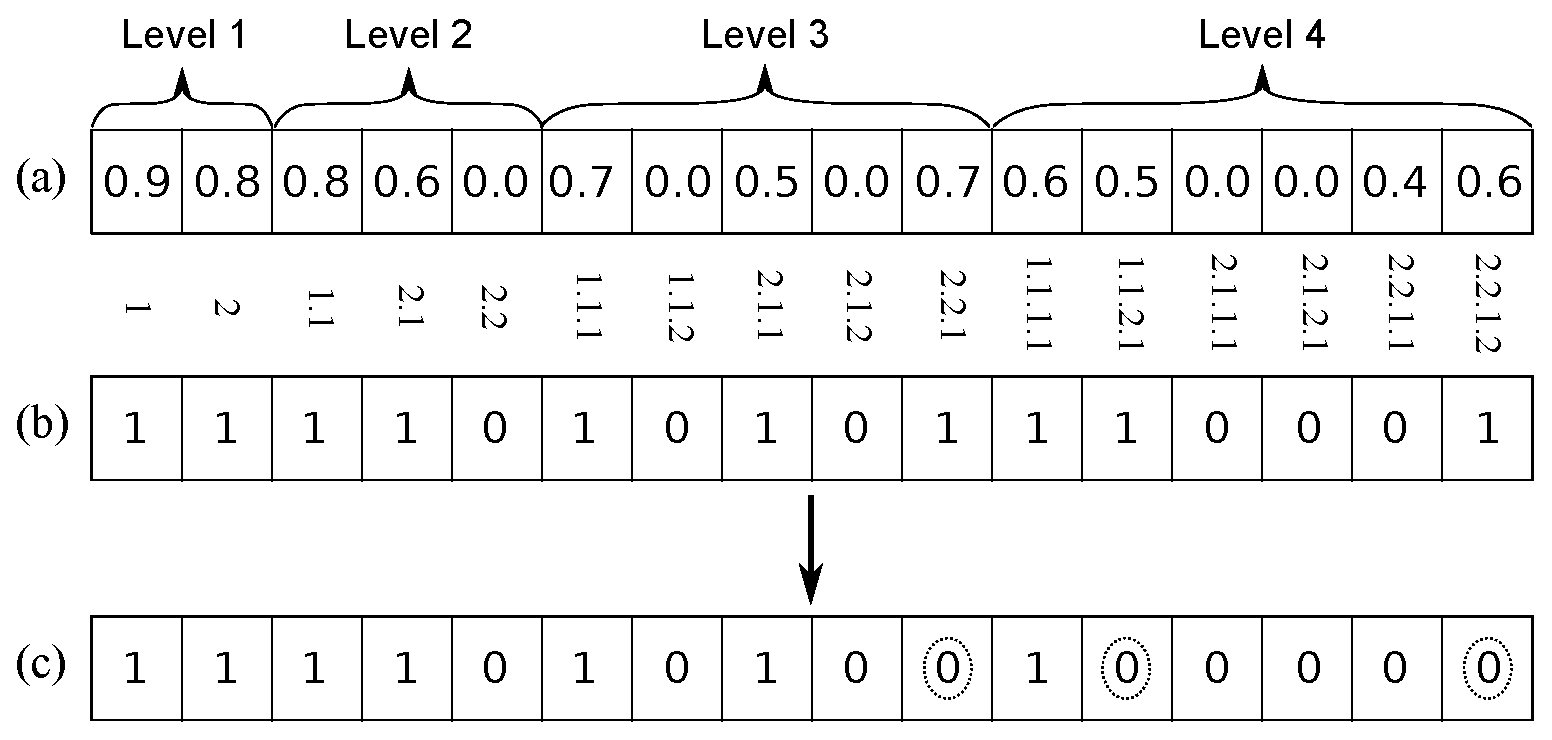
\includegraphics[scale=0.33]{VectorClasses}
%       \caption{Example of the class-predicted vector provided by HMC-LMLP. (a) Outputs from the neurons; (b) Prediction after applying a threshold value of 0.5; (c) Final classification after correcting inconsistencies.}
%       \label{fig:vectorClasses}
%\end{figure}

\subsection{Computational complexity}

Each MLP used in HMC-LMLP-Comp has a complexity of $\mathcal{O}(W_l)$, with $W_l$ being the number of weights and biases of the MLP associated with level $l$. Let $A$ be the number of attributes in the dataset, $H_l$ be the number of hidden neurons of the MLP associated with level $l$, and $O_l$ be the number of output neurons of the MLP associated with level $l$. We can thus define $W_1$ as $(A + 1) \times H_1 + (H_1 + 1) \times O_1$. From the second level onwards, $W_l$ is defined as $(O_{l-1} + A + 1) \times H_l + (H_l + 1) \times O_l$. The training cost of each MLP associated with level $l$ in HMC-LMLP-Comp is then $\mathcal{O}(W_l \times m_l \times n)$, with $m_l$ being the number of training instances assigned to classes belonging to level $l$, and $n$ the number of training epochs. In HMC-LMLP-NoComp, the computational cost is smaller, since the class labels are not used to augment the feature vectors.
\section{Experiments}\label{sec:experiments}

In this section, we present the experiments that were carried out to compare the prediction performance achieved by HMC-LMLP's versions and the state-of-the-art HMC~algorithms. We also present the datasets, parameters, and the evaluation measure that were employed in the experiments.

\subsection{Datasets}

We make use of ten freely available\footnote{\url{http://www.cs.kuleuven.be/~dtai/clus/hmcdatasets.html}} datasets related to protein function prediction. These datasets are related to issues like phenotype data and gene expression levels. Table~\ref{tab:datasets} presents the main characteristics of the training, validation, and test datasets. A description of each dataset can be found in \cite{Vens2008}.

Considering that there is no level definition in DAG structures (a class can be located at different levels depending on which hierarchical path is chosen from the root node to the class), we defined the depth of a class in a DAG structure as the deepest path from the class to the root node. This is necessary for the application of HMC-LMLP, since the method requires a clear separation of classes in levels. We chose the deepest path as the definition of depth because it guarantees that when a class is located in a level $l$, all its superclasses will be located in levels shallower~than~$l$. With this depth definition, each hierarchy ended up with 13~levels.

\begin{table*}[htpb]
\centering
\setlength{\tabcolsep}{6pt}
\caption{Summary of the datasets: number of attributes ($|A|$), number of classes ($|C|$), number of classes per level (Classes per level), total number of instances (Total) and number of multi-label instances~(Multi).}
\scriptsize
\begin{tabular*}{\textwidth}
    {@{\extracolsep{\fill}}lccccccccc}
\toprule
\multirow{2}{*}{Dataset} & \multirow{2}{*}{$|A|$}  & \multirow{2}{*}{$|C|$} & \multirow{2}{*}{Classes per level} & \multicolumn{ 2}{c}{Training} & \multicolumn{ 2}{c}{Valid} &  \multicolumn{ 2}{c}{Test} \\ 
 & & & & Total & Multi & Total & Multi & Total & Multi \\ \midrule
 
Cellcycle &  77  &  4122  & 33/155/394/597/929/779/631/335/171/63/21/5/9 & 1625  & 1625   &  848  &  848  &  1278  & 1278   \\

Church    &  27  &  4122  & 33/155/394/597/929/779/631/335/171/63/21/5/9 & 1627  &  1627  &  844  & 844  &  1278  & 1278 \\

Derisi    &  63  &  4116  & 33/155/394/596/927/778/630/334/171/63/21/5/9 & 1605  & 1605   &  842  &  842  &  1272  &  1272 \\

Eisen     &  79  &  3570  & 33/149/360/524/786/679/539/271/141/55/19/5/9 & 1055  &  1055  &  528  &  528  &  835  & 835 \\
  
Expr      &  551 &  4128  & 33/155/394/599/932/780/631/335/171/63/21/5/9 & 1636  &  1636  &  849  &  849  &  1288  & 1288 \\
  
Gasch1    &  173 &  4122  & 33/155/394/597/929/779/631/335/171/63/21/5/9 & 1631  &  1631  &  846  &  846  &  1281  & 1281 \\
  
Gasch2    &  52  &  4128  & 33/155/394/599/932/780/631/335/171/63/21/5/9 & 1636  &  1636  &  849  &  849  &  1288  & 1288 \\
  
Pheno     &  69  &  3124  & 33/145/332/489/670/568/460/236/114/49/18/4/6 & 653  &  653  &  352  &  352  &  581  & 581 \\
    
Seq       &  478 &  4130 & 33/155/394/599/932/780/633/335/171/63/21/5/9 & 1692  &  1692  &  876  &  876  &  1332   &  1332 \\
  
Spo       &  80  & 4116  & 33/155/394/596/927/778/630/334/171/63/21/5/9 & 1597  &  1597  & 837  &  837  &  1263  & 1263 \\
 
\bottomrule  
  
\end{tabular*}
\label{tab:datasets}
\end{table*}

We performed a pre-processing step before running HMC-LMLP over these datasets, in which all nominal attribute values were transformed into numeric values using the one-attribute-per-value approach. In this paper, instead of using $0$s and $1$s, the nominal attributes were assigned $-1$ (absence) and $1$ (presence), which are better suited for training neural networks \cite{Haykin1999}. The attributes were then standardized (mean $0$ and variance $1$). Additionally, all missing values for nominal and numeric attributes were replaced, respectively, by their mode and mean values.

\subsection{Evaluation Measure}

The outputs of HMC-LMLP, for each class, are real values between 0 and 1. The same is true for the literature methods. Thus, in order to obtain the final predictions, a threshold value was further employed. When classifying an instance, if the corresponding output value for a given class is greater than or equal to the threshold, the instance is assigned to the class, otherwise it is not.

The choice of the ``optimal" threshold value is a difficult task, since low threshold values lead to many classes being assigned to each instance, resulting in high recall and low precision. On the other hand, large threshold values lead to very few instances being classified, resulting in high precision and low recall. To deal with this problem, we make use of precision-recall curves (PR-curves) as the evaluation measure for the experiments. To obtain a PR-curve, different thresholds between [0,1] are applied to the outputs of the methods, and thus different values of precision and recall are obtained, one for each threshold value. Each threshold then represents a point within the PR-space. The union of these points form a PR-curve, and the area under the curve is calculated. All methods are thus compared based on their areas under~the~PR-curves.

More specifically, we employed the area under the average PR-curve ($AU(\overline{PRC})$). Given a threshold value, a precision-recall point ($\overline{Prec},\overline{Rec}$) in the PR-space can be obtained through Equations~(\ref{eq:prec})~and~(\ref{eq:reca}). They correspond to the micro-average of precision and recall.

\begin{multicols}{2}
	\begin{equation}
		\overline{Prec} = \frac{\sum_i TP_i}{\sum_i TP_i + \sum_i FP_i}
		\label{eq:prec}
	\end{equation}

	\begin{equation}
		\overline{Rec} = \frac{\sum_i TP_i}{\sum_i TP_i + \sum_i FN_i}
		\label{eq:reca}
	\end{equation}
\end{multicols}

To verify the significance of the results, we employed the Friedman and Nemenyi statistical tests, recommended for comparisons involving many classifiers and several datasets \cite{Demsar2006}. We adopted a confidence level of 95\% in the statistical~tests. As in \cite{Vens2008} and \cite{Otero2010}, 2/3 of each dataset were used for inducing the classification models and 1/3 for~test. We used the same data partitions suggested in \cite{Vens2008}.

\subsection{Parameters}

We investigate the performance of HMC-LMLP using the conventional Back-propagation algorithm (Bp) \cite{Rumelhart1986}, and the Resilient Back-propagation (Rprop)~\cite{Riedmiller1993}.

The HMC-LMLP parameters were optimized using the Eisen validation dataset. This dataset was selected because it was one of the datasets where Clus-HMC obtained its best performance (0.380), and also because it has a relatively small number of attributes, which allows to run several experiments in a reasonable amount of time. The following parameters were optimized: (i) number of neurons in each hidden layer (beginning with the hidden layer of the MLP network associated with the first hierarchical level, and finishing with the hidden layer of the MLP network associated with the last level), (ii) the learning rate and momentum constant used in the Back-propagation algorithm, and (iii) the range of values used to initialize the neural network's weights. %To reduce the influence of parameter selection in the MLP predictive performance, the number of hidden neurons was set as a fraction of the number of input~attributes.
We executed HMC-LMLP over the validation dataset using different sets of parameter values. We employed different initial weight values, number of hidden neurons, learning rates, and momentum constants. We did not use all possible sets of values due to the large number of possibilities.

\sloppy
For the initial weights, we noticed that the larger their values, the more likely was overfitting to occur (a better performance on more frequent classes but a worse overall prediction performance). We varied the initial weights by randomly selecting them initially from [-0.1,0.1], but gradually increasing the range to [-1,1]. We tested a limited number of neurons for each hidden layer, beginning with 1.0/1.0/0.95/0.9/0.85/0.8/0.75/0.7/0.65/0.6/0.55/0.5/0.45 neurons in each layer and gradually decreasing these values. These hidden neuron numbers represent the fraction of the total number of network inputs. Thus, if a neural network has 100 inputs, the value 0.6 means that it has actually 60 hidden neurons. Considering the learning rate and momentum, we started our experiments with the same default values used in the Weka toolkit~\cite{Weka}, in which the learning rate is set to 0.3 and the momentum to 0.2. We gradually decreased these values and noticed that the neural networks became less prone to overfitting as these values decreased. The final parameters obtained for HMC-LMLP after the preliminary experiments are listed~next.

\begin{itemize}
    \sloppy
	\item Number of hidden neurons per level (fraction of the total number of network inputs): 0.65/0.65/0.6/0.55/0.5/0.45/0.4/0.35/0.3/0.25/0.2/0.15/\\0.1;
	
	\item Learning rate and momentum constant used in Back-propagation for hidden and output layers: $\{0.05, 0.03\}$ and $\{0.03, 0.01\}$, respectively;

	\item Initial weights of the neural networks: within [-0.1,0.1];
	
	\item Parameter values of the Rprop algorithm: initial Delta ($\Delta_0$) = 0.1, maximum Delta ($\Delta_{max}$) = 50.0, minimum Delta ($\Delta_{min}$) = $1e^{-6}$, increase factor ($\eta^+$) = 1.2, and decrease factor ($\eta^-$) = 0.5. 
\end{itemize}

We would like to point out that we decreased the number of hidden neurons of the neural networks as the hierarchical levels became deeper. Our intention was to avoid overfitting, since the number of training instances is smaller for the networks associated with deeper hierarchical levels. The first two values (0.65/0.65) are the same because all instances are classified in classes belonging to the first and second levels. The Rprop parameter values were the ones suggested in \cite{Riedmiller1993}.

\subsection{Results}

Table~\ref{tab:prcurves} presents the PR-curves for the HMC-LMLP's versions and the literature methods. We refer to the HMC-LMLP versions as Bp-Comp (Back-propagation with classes augmenting the feature vectors), Bp-NoComp (Back-propagation with no augmentation), Rprop-Comp (Resilient Back-propagation with classes augmenting the feature vectors), and Rprop-NoComp (Resilient Back-propagation with no augmentation).

The results for HMC-LMLP and {\it hm}Ant-Miner are the mean and standard deviation over 10 executions. Each HMC-LMLP execution was performed with randomly initialized weights. Clus-HMC, Clus-HSC, and Clus-SC are deterministic algorithms, and thus require a single execution. We highlight the best absolute~values.

\begin{table*}[ht]
\scriptsize
\centering
\setlength{\tabcolsep}{3pt}
%\renewcommand{\arraystretch}{1.3}
\caption{$AU(\overline{PRC})$ values obtained}
\begin{tabular*}{\textwidth}
    {@{\extracolsep{\fill}}lcccccccc}
\toprule
Dataset & Bp-Comp  & Bp-NoComp & Rprop-Comp & Rprop-NoComp & Clus-HMC & Clus-HSC & Clus-SC & {\it hm}Ant-Miner \\ 
\midrule
 
Cellcycle & 0.352 $\pm$ 0.0025 & 0.359 $\pm$ 0.0007 & 0.357 $\pm$ 0.001 & 0.365 $\pm$ 0.001 & 0.357 & {\bf 0.371} & 0.252 & 0.325 $\pm$ 0.0079\\

Church  & 0.336 $\pm$ 0.0015 & 0.340 $\pm$ 0.0011 & 0.341 $\pm$ 0.003 & 0.347 $\pm$ 0.001 & 0.348 & {\bf 0.397} & 0.289 & 0.334 $\pm$ 0.0010\\

Derisi    & 0.336 $\pm$ 0.0013 & 0.345 $\pm$ 0.0006 & 0.336 $\pm$ 0.002 & 0.349 $\pm$ 0.001 & {\bf 0.355} & 0.349 & 0.218 & 0.321 $\pm$ 0.0068\\

Eisen     & 0.393 $\pm$ 0.0014 & 0.395 $\pm$ 0.0012 & 0.396 $\pm$ 0.003 & {\bf 0.403 $\pm$ 0.001} & 0.380 & 0.365 & 0.270 & 0.373 $\pm$ 0.0110\\

Gasch1  & 0.373 $\pm$ 0.0029 & 0.378 $\pm$ 0.0012 & 0.372 $\pm$ 0.004 & {\bf 0.384 $\pm$ 0.001} & 0.371 & 0.351 & 0.239 & 0.352 $\pm$ 0.0082\\

Gasch2  & 0.359 $\pm$ 0.0019 & 0.362 $\pm$ 0.0012 & 0.359 $\pm$ 0.003 & 0.369 $\pm$ 0.001 & 0.365 & {\bf 0.378} & 0.267 & 0.334 $\pm$ 0.0165\\

Pheno    & 0.315 $\pm$ 0.0025 & 0.322 $\pm$ 0.0011 & 0.316 $\pm$ 0.002 & 0.325 $\pm$ 0.002 & 0.337 & {\bf 0.416} & 0.316 & 0.336 $\pm$ 0.0017\\

Spo        & 0.334 $\pm$ 0.0021 & 0.340 $\pm$ 0.0007 & 0.332 $\pm$ 0.003 & 0.345 $\pm$ 0.001 & 0.352 & {\bf 0.371} & 0.213 & 0.329 $\pm$ 0.0078\\

Expr       & 0.369 $\pm$ 0.0031 & 0.371 $\pm$ 0.0014 & 0.373 $\pm$ 0.003 & {\bf 0.384 $\pm$ 0.002} & 0.368 & 0.351 & 0.249 & 0.343 $\pm$ 0.0066\\

Seq        & 0.368 $\pm$ 0.0034 & 0.368 $\pm$ 0.0018 & 0.375 $\pm$ 0.003 & 0.384 $\pm$ 0.002 & {\bf 0.386} & 0.282 & 0.197 & 0.371 $\pm$ 0.0069\\

\midrule
Average & 0.355 & 0.358 & 0.356 & {\bf 0.365} & 0.362 & 0.363 & 0.251 & 0.342           \\ 
\bottomrule
\end{tabular*}
\label{tab:prcurves}
\end{table*}

We also compared the HMC methods considering specific classes with the goal of examining their behavior when predicting classes in different hierarchical levels. Since Clus-HMC is considered to be the state-of-the-art method, we performed the comparisons in the Seq dataset, in which Clus-HMC showed the best results according to Table~\ref{tab:prcurves}.

We selected, for each level, the three classes where Clus-HMC obtained its best results. We went down until the seventh hierarchical level. Results are shown in Table~\ref{tab:classesSeq}. The best absolute values are highlighted.

\begin{table*}[ht]
\scriptsize
\centering
\setlength{\tabcolsep}{3pt}
%\renewcommand{\arraystretch}{1.3}
\caption{Best $AU(\overline{PRC})$ obtained in specific classes for the Seq dataset.}
\begin{tabular*}{\textwidth}
    {@{\extracolsep{\fill}}clccccccccc}
\toprule
Level & Classes  & Bp-Comp & Bp-NoComp & Rprop-Comp & Rprop-NoComp & Clus-HMC & Clus-HSC & Clus-SC & {\it hm}Ant-Miner  \\
 \midrule
1 & GO:0044464  & 0.963 $\pm$ 0.006 & {\bf 0.966 $\pm$ 0.002} & 0.965 $\pm$ 0.002 & 0.964 $\pm$ 0.006 & 0.960 & 0.951 & 0.951 & 0.953 $\pm$ 0.0054 \\
1 & GO:0009987  & 0.869 $\pm$ 0.005 & 0.868 $\pm$ 0.004 & 0.870 $\pm$ 0.004 & {\bf 0.873 $\pm$ 0.006} & 0.872 & 0.844 & 0.844 & 0.870 $\pm$ 0.0072 \\
1 & GO:0008152  & 0.791 $\pm$ 0.010 & 0.790 $\pm$ 0.008 & {\bf 0.797 $\pm$ 0.007} & 0.796 $\pm$ 0.006 & 0.774 & 0.700 & 0.700 & 0.730 $\pm$ 0.0098 \\

2 & GO:0044424  & 0.934 $\pm$ 0.002 & {\bf 0.937 $\pm$ 0.003} & 0.936 $\pm$ 0.003 & 0.935 $\pm$ 0.003 & 0.922 & 0.897 & 0.894 & 0.916 $\pm$ 0.0051 \\
2 & GO:0044237  & 0.723 $\pm$ 0.011 & 0.734 $\pm$ 0.009 & 0.734 $\pm$ 0.007 & {\bf 0.742 $\pm$ 0.009} & 0.714 & 0.694 & 0.686 & 0.685 $\pm$ 0.0123 \\
2 & GO:0044238  & 0.690 $\pm$ 0.012 & 0.691 $\pm$ 0.010 & {\bf 0.702 $\pm$ 0.009} & 0.701 $\pm$ 0.006 & 0.664 & 0.632 & 0.634 & 0.651 $\pm$ 0.0142 \\

3 & GO:0044446  & {\bf 0.691 $\pm$ 0.007} & 0.687 $\pm$ 0.007 & 0.677 $\pm$ 0.011 & 0.674 $\pm$ 0.005 & 0.649 & 0.610 & 0.564 & 0.615 $\pm$ 0.0162 \\
3 & GO:0044444  & 0.648 $\pm$ 0.014 & {\bf 0.652 $\pm$ 0.009} & 0.630 $\pm$ 0.014 & 0.636 $\pm$ 0.008 & 0.629 & 0.546 & 0.530 & 0.570 $\pm$ 0.0083 \\
3 & GO:0043229  & 0.591 $\pm$ 0.008 & 0.597 $\pm$ 0.007 & {\bf 0.601 $\pm$ 0.007} & 0.595 $\pm$ 0.006 & 0.584 & 0.554 & 0.547 & 0.561 $\pm$ 0.0109 \\

4 & GO:0043231  & 0.558 $\pm$ 0.009 & 0.562 $\pm$ 0.008 & {\bf 0.567 $\pm$ 0.008} & 0.561 $\pm$ 0.004 & 0.535 & 0.500 & 0.485 & 0.514 $\pm$ 0.0081 \\
4 & GO:0044428  & 0.491 $\pm$ 0.019 & 0.495 $\pm$ 0.015 & 0.496 $\pm$ 0.013 & {\bf 0.497 $\pm$ 0.019} & 0.446 & 0.353 & 0.346 & 0.409 $\pm$ 0.0256 \\
4 & GO:0044267  & 0.428 $\pm$ 0.015 & {\bf 0.460 $\pm$ 0.010} & 0.450 $\pm$ 0.011 & 0.458 $\pm$ 0.012 & 0.383 & 0.337 & 0.329 & 0.376 $\pm$ 0.0240 \\

5 & GO:0006412  & 0.684 $\pm$ 0.014 & {\bf 0.684 $\pm$ 0.012} & 0.664 $\pm$ 0.018 & 0.678 $\pm$ 0.012 & 0.491 & 0.440 & 0.501 & 0.435 $\pm$ 0.0279 \\
5 & GO:0005634  & 0.321 $\pm$ 0.013 & 0.323 $\pm$ 0.017 & 0.317 $\pm$ 0.009 & 0.320 $\pm$ 0.011 & {\bf 0.327} & 0.241 & 0.283 & 0.322 $\pm$ 0.0192 \\
5 & GO:0005739  & 0.395 $\pm$ 0.016 & {\bf 0.403 $\pm$ 0.007} & 0.390 $\pm$ 0.012 & 0.386 $\pm$ 0.014 & 0.308 & 0.284 & 0.310 & 0.244 $\pm$ 0.0096 \\

6 & GO:0045449  & {\bf 0.239 $\pm$ 0.020} & 0.226 $\pm$ 0.016 & 0.191 $\pm$ 0.013 & 0.218 $\pm$ 0.023 & 0.167 & 0.106 & 0.127 & 0.188 $\pm$ 0.0267 \\
6 & GO:0017111  & 0.115 $\pm$ 0.024 & 0.122 $\pm$ 0.028 & 0.301 $\pm$ 0.033 & {\bf 0.304 $\pm$ 0.030} & 0.134 & 0.190 & 0.200 & 0.071 $\pm$ 0.0053 \\
6 & GO:0043687  & 0.227 $\pm$ 0.027 & 0.218 $\pm$ 0.026 & {\bf 0.236 $\pm$ 0.026} & 0.235 $\pm$ 0.026 & 0.105 & 0.096 & 0.120 & 0.115 $\pm$ 0.0136 \\

7 & GO:0006355  & {\bf 0.233 $\pm$ 0.017} & 0.225 $\pm$ 0.016 & 0.183 $\pm$ 0.010 & 0.209 $\pm$ 0.021 & 0.173 & 0.100 & 0.117 & 0.174 $\pm$ 0.0217 \\
7 & GO:0016568  & 0.099 $\pm$ 0.014 & 0.092 $\pm$ 0.012 & 0.093 $\pm$ 0.006 & {\bf 0.121 $\pm$ 0.011} & 0.094 & 0.051 & 0.058 & 0.079 $\pm$ 0.0128 \\
7 & GO:0000723  & 0.081 $\pm$ 0.008 & {\bf 0.086 $\pm$ 0.011} & 0.082 $\pm$ 0.012 & 0.081 $\pm$ 0.009 & 0.085 & 0.064 & 0.056 & 0.082 $\pm$ 0.0104 \\
\midrule
& Average & 0.513 & 0.515 & 0.518 & {\bf 0.523} & 0.477 & 0.438 & 0.442 & 0.455        \\
\bottomrule
\end{tabular*}
\label{tab:classesSeq}
\end{table*}

\section{Discussion}\label{sec:discussion}

According to Table~\ref{tab:prcurves}, the best results were obtained by Rprop-NoComp, Clus-HMC and Clus-HSC. We can see that using the true classes to augment the feature vectors did not improve the classification results when compared to the HMC-LMLP version that does not use the augmentation process. We believe there are two reasons that may have harmed Bp(Rprop)-Comp's performance: (i) adapting the DAG hierarchy, and (ii) using different values to augment the feature vectors during the training and test phases.

Regarding the adaptation made in the DAG hierarchies, Bp-Comp and Rprop-Comp could have achieved better performance if all relationships between classes had been available during training. Recall we had to adapt the DAG hierarchy to define the depth of a class as being the number of edges in the longest path between class and root node. For that reason, many hierarchical relationships between classes were not considered during the training phase. Figure~\ref{fig:hrelationships} illustrates a scenario that explains this rationale.

\begin{figure}[htbp]
       \centering
       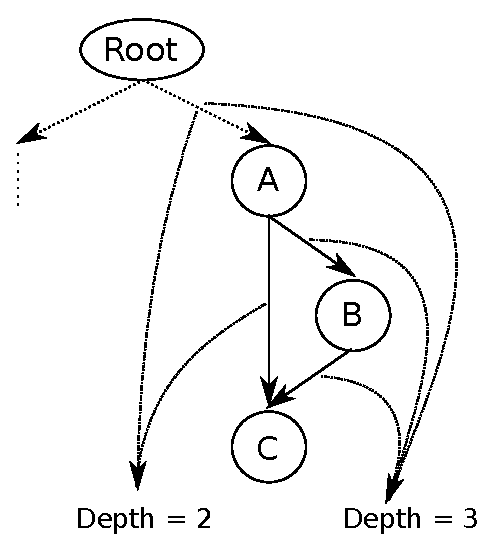
\includegraphics[scale=0.5]{hrelationships}
       \caption{Illustrative example of different depths for the same class.}
       \label{fig:hrelationships}
\end{figure}

Following the scenario presented in Figure~\ref{fig:hrelationships}, consider that a training instance is assigned to paths A.C and A.B.C, and that class C is a direct subclass of both classes A and B. In this scenario, there are two possible depths for class C: 2 (A.C) and 3 (A.B.C). In the adaptation process we have proposed, class C is defined as belonging to the third level. In this case, when training an MLP for the third level, we consider class C as subclass of class B alone. Thus, when training a neural network to predict class C (third level), we are not using the information related to all its superclasses (classes A and B) as inputs. Only class B is considered.

The different values that are used when augmenting the feature vectors may also have harmed the performance of Bp-Comp and Rprop-Comp. Recall that when training an MLP for level $l$, we make use of the true labels of the training instances (values 0 or 1) at level $l-1$ to augment their feature vectors. However, the true labels are not available during test. Thus, the predictions made by the neural network at level $l-1$ (values [0,1]) were used instead. Therefore, each MLP was trained using 0 or 1 values for augmenting the feature vectors during training, but were tested with real values in the interval [0,1].

Comparing the Bp and Rprop algorithms, note that the Rprop versions of HMC-LMLP provided better predictive performance than the Bp versions. These results suggest that Rprop copped better with the greater number of attributes, which increased considerably due to the augmentation process. 

\begin{figure}[!htpb]
 \centering 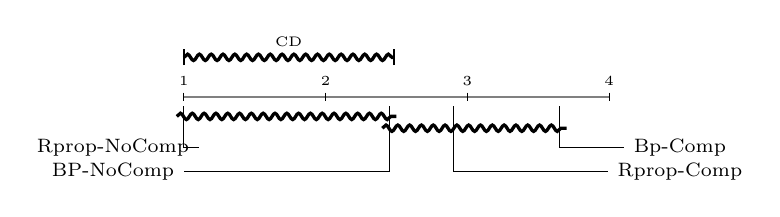
\begin{tikzpicture}[xscale=1.8]
\node (Label) at  (01.7400,0.7) {\tiny{CD}}; % the label
\draw[decorate,decoration={snake,amplitude=.4mm,segment length=1.5mm,post length=0mm}, very thick, color = black](01.0000, 0.5) -- (02.4800, 0.5);
\foreach \x in {01.0000,02.4800} \draw[thick,color = black] (\x, 0.4) -- (\x, 0.6);

\draw[gray, thick](01.0000, 0) -- (04.0000, 0);
\foreach \x in {01.0000,02.0000,03.0000,04.0000}\draw (\x cm,1.5pt) -- (\x cm, -1.5pt);
\node (Label) at (01.0000,0.2) {\tiny{1}};
\node (Label) at (02.0000,0.2) {\tiny{2}};
\node (Label) at (03.0000,0.2) {\tiny{3}};
\node (Label) at (04.0000,0.2) {\tiny{4}};
\draw[decorate,decoration={snake,amplitude=.4mm,segment length=1.5mm,post length=0mm}, very thick, color = black](00.9500,-00.2500) -- ( 02.5000,-00.2500);
\draw[decorate,decoration={snake,amplitude=.4mm,segment length=1.5mm,post length=0mm}, very thick, color = black](02.4000,-00.4000) -- ( 03.7000,-00.4000);
\node (Point) at (01.0000, 0){};  \node (Label) at (0.5,-00.6500){\scriptsize{Rprop-NoComp}}; \draw (Point) |- (Label);
\node (Point) at (02.4500, 0){};  \node (Label) at (0.5,-00.9500){\scriptsize{BP-NoComp}}; \draw (Point) |- (Label);
\node (Point) at (03.6500, 0){};  \node (Label) at (4.5,-00.6500){\scriptsize{Bp-Comp}}; \draw (Point) |- (Label);
\node (Point) at (02.9000, 0){};  \node (Label) at (4.5,-00.9500){\scriptsize{Rprop-Comp}}; \draw (Point) |- (Label);
\end{tikzpicture}
\caption{Critical diagram presenting results of the 4 HMC-LMLP's versions.}
\label{fig:cdNN}
\end{figure}

Figure~\ref{fig:cdNN} shows the results of the statistical tests regarding the 4 HMC-LMLP's versions. Note that Rprop-NoComp outperforms most versions of HMC-LMLP with statistical significance. The difference for BP-NoComp is within the limit of the critical difference. The tests confirm that Rprop was the best learning algorithm in both scenarios (with and without augmentation). 


Figure~\ref{fig:cdAll} presents the results of the statistical tests regarding the best version of HMC-LMLP (Rprop-NoComp) and the 4 baseline methods (Clus-HMC, Clus-HSC, Clus-SC, and \textit{hm}Ant-Miner). Clus-HMC provides the lowest average rank (2.0), whereas Rprop-NoComp provides the second lowest (2.15) followed by Clus-HSC (2.25). Note that the difference in average rank among these three methods is very small, and indeed it is deemed as insignificant by the statistical tests. The performance achieved by \textit{hm}Ant-Miner (average rank of 3.6) and Clus-SC (average rank of 5.0) is considerably lower than the best ranked methods. Even though \textit{hm}Ant-Miner is within the limit of the critical difference, Clus-SC is out of the significance margin, which means it is outperformed by the first three methods with statistical significance.

\begin{figure}[!htpb]
 \centering 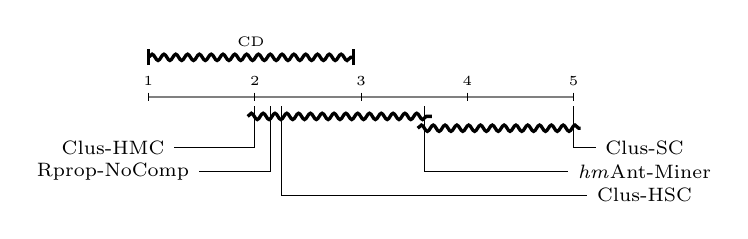
\begin{tikzpicture}[xscale=1.8]
\node (Label) at  (01.4734,0.7) {\tiny{CD}}; % the label
\draw[decorate,decoration={snake,amplitude=.4mm,segment length=1.5mm,post length=0mm}, very thick, color = black](00.7500, 0.5) -- (02.1967, 0.5);
\foreach \x in {00.7500,02.1967} \draw[thick,color = black] (\x, 0.4) -- (\x, 0.6);

\draw[gray, thick](00.7500, 0) -- (03.7500, 0);
\foreach \x in {00.7500,01.5000,02.2500,03.0000,03.7500}\draw (\x cm,1.5pt) -- (\x cm, -1.5pt);
\node (Label) at (00.7500,0.2) {\tiny{1}};
\node (Label) at (01.5000,0.2) {\tiny{2}};
\node (Label) at (02.2500,0.2) {\tiny{3}};
\node (Label) at (03.0000,0.2) {\tiny{4}};
\node (Label) at (03.7500,0.2) {\tiny{5}};
\draw[decorate,decoration={snake,amplitude=.4mm,segment length=1.5mm,post length=0mm}, very thick, color = black](01.4500,-00.2500) -- ( 02.7500,-00.2500);
\draw[decorate,decoration={snake,amplitude=.4mm,segment length=1.5mm,post length=0mm}, very thick, color = black](02.6500,-00.4000) -- ( 03.8000,-00.4000);
\node (Point) at (01.5000, 0){};  \node (Label) at (0.5,-00.6500){\scriptsize{Clus-HMC}}; \draw (Point) |- (Label);
\node (Point) at (01.6125, 0){};  \node (Label) at (0.5,-00.9500){\scriptsize{Rprop-NoComp}}; \draw (Point) |- (Label);
\node (Point) at (03.7500, 0){};  \node (Label) at (4.25,-00.6500){\scriptsize{Clus-SC}}; \draw (Point) |- (Label);
\node (Point) at (02.7000, 0){};  \node (Label) at (4.25,-00.9500){\scriptsize{\textit{hm}Ant-Miner}}; \draw (Point) |- (Label);
\node (Point) at (01.6875, 0){};  \node (Label) at (4.25,-01.2500){\scriptsize{Clus-HSC}}; \draw (Point) |- (Label);
\end{tikzpicture}
\caption{Critical diagram presenting results of the best HMC-LMLP network and the baseline algorithms.}
\label{fig:cdAll}
\end{figure}

Considering the results in specific classes (Table~\ref{tab:classesSeq}), HMC-LMLP provided the best results in the great majority of the classes. These results are quite unexpected, given that Clus-HMC achieved a better overall performance than Bp-Comp, Bp-NoComp and Rprop-Comp (Table~\ref{tab:prcurves}). Notwithstanding, we verified that from the 2849 classes that belong to the test dataset, Clus-HMC provided the best results for 2192, whereas the HMC-LMLP's versions achieved the best results in a much smaller number of classes. Hence the results of Clus-HMC in Table~\ref{tab:prcurves}.

The PR-curves obtained for datasets Eisen and Seq are depicted in Figure~\ref{fig:prcurves}. These datasets are the ones where Clus-HMC obtained its best results. We compared the PR-curves of the literature methods with the PR-curve obtained by Rprop-NoComp, since it was the best among the HMC-LMLP's versions. The PR-curves shown for HMC-LMLP and {\it hm}Ant-Miner are those from the executions in which they obtained the best results in the validation data. We can see that Clus-HMC, Clus-HSC and HMC-LMLP are quite even performance-wise.

\begin{figure*}[ht]
        \centering
        \begin{subfigure}[b]{0.3\textwidth}
                \centering
                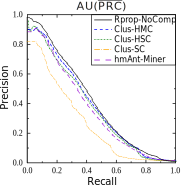
\includegraphics[scale=1.1]{eisen}
                \caption{Eisen dataset}
                \label{fig:eisenTree}
        \end{subfigure}
		\qquad\qquad\qquad
        \begin{subfigure}[b]{0.3\textwidth}
                \centering
                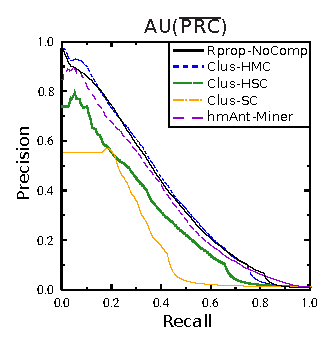
\includegraphics[scale=1.1]{seq}
                \caption{Seq dataset}
                \label{fig:seqTree}
        \end{subfigure}
        \caption{PR-curves of Rprop-NoComp, Clus-HMC, CLus-HSC, Clus-SC, and {\it hm}Ant-Miner.}
        \label{fig:prcurves}
\end{figure*}
\section{Conclusion}\label{sec:conclusion}
In this paper, we presented {\bf H}ierarchical {\bf M}ulti-Label {\bf C}lassification with {\bf L}ocal {\bf M}ulti-{\bf L}ayer {\bf P}erceptron (HMC-LMLP), which associates an MLP to each level of a DAG-structure class hierarchy. HMC-LMLP employs the Local Classifier per Level (LCL)~\cite{Silla2010} strategy, complementing the feature vectors of the instances with their true classes, in order to make use of local information within each level of the hierarchy. With this, we try to avoid problems such as the loss of label dependency during training.

We tested HMC-LMLP on ten datasets related to protein function prediction, in which the protein functions were organized following the Gene Ontology. We compared its performance against the state-of-the-art methods in the literature of HMC, and the empirical analysis indicates that HMC-LMLP matches the state-of-the-art methods in terms of predictive performance, often presenting better results in specific classes of the DAG hierarchy.

We also showed that the use of true labels to complement the feature vectors did not improve the classification performance. We also showed that this may have happened because the adaptation performed in the DAG taxonomies, which resulted in no use of the complete information regarding parent-child class relationship.

As future work, we intend to investigate other neural network training algorithms, such as Extreme Learning Machines~\cite{Huang2004} and Improved Resilient Back-propagation~\cite{Igel2000}. We will also investigate alternatives to adapt the DAG taxonomies to be used with HMC-LMLP, trying to overcome the disadvantages of the currently used adaptation. Other strategies for correct inconsistencies in the prediction will also be tried. Finally, we plan to incorporate other knowledge source in the training process, such as protein-protein interactions networks, and also use HMC-LMLP in other application domains, such as text classification.

% An example of a floating figure using the graphicx package.
% Note that \label must occur AFTER (or within) \caption.
% For figures, \caption should occur after the \includegraphics.
% Note that IEEEtran v1.7 and later has special internal code that
% is designed to preserve the operation of \label within \caption
% even when the captionsoff option is in effect. However, because
% of issues like this, it may be the safest practice to put all your
% \label just after \caption rather than within \caption{}.
%
% Reminder: the "draftcls" or "draftclsnofoot", not "draft", class
% option should be used if it is desired that the figures are to be
% displayed while in draft mode.
%
%\begin{figure}[!t]
%\centering
%\includegraphics[width=2.5in]{myfigure}
% where an .eps filename suffix will be assumed under latex, 
% and a .pdf suffix will be assumed for pdflatex; or what has been declared
% via \DeclareGraphicsExtensions.
%\caption{Simulation Results}
%\label{fig_sim}
%\end{figure}

% Note that IEEE typically puts floats only at the top, even when this
% results in a large percentage of a column being occupied by floats.


% An example of a double column floating figure using two subfigures.
% (The subfig.sty package must be loaded for this to work.)
% The subfigure \label commands are set within each subfloat command, the
% \label for the overall figure must come after \caption.
% \hfil must be used as a separator to get equal spacing.
% The subfigure.sty package works much the same way, except \subfigure is
% used instead of \subfloat.
%
%\begin{figure*}[!t]
%\centerline{\subfloat[Case I]\includegraphics[width=2.5in]{subfigcase1}%
%\label{fig_first_case}}
%\hfil
%\subfloat[Case II]{\includegraphics[width=2.5in]{subfigcase2}%
%\label{fig_second_case}}}
%\caption{Simulation results}
%\label{fig_sim}
%\end{figure*}
%
% Note that often IEEE papers with subfigures do not employ subfigure
% captions (using the optional argument to \subfloat), but instead will
% reference/describe all of them (a), (b), etc., within the main caption.


% An example of a floating table. Note that, for IEEE style tables, the 
% \caption command should come BEFORE the table. Table text will default to
% \footnotesize as IEEE normally uses this smaller font for tables.
% The \label must come after \caption as always.
%
%\begin{table}[!t]
%% increase table row spacing, adjust to taste
%\renewcommand{\arraystretch}{1.3}
% if using array.sty, it might be a good idea to tweak the value of
% \extrarowheight as needed to properly center the text within the cells
%\caption{An Example of a Table}
%\label{table_example}
%\centering
%% Some packages, such as MDW tools, offer better commands for making tables
%% than the plain LaTeX2e tabular which is used here.
%\begin{tabular}{|c||c|}
%\hline
%One & Two\\
%\hline
%Three & Four\\
%\hline
%\end{tabular}
%\end{table}


% Note that IEEE does not put floats in the very first column - or typically
% anywhere on the first page for that matter. Also, in-text middle ("here")
% positioning is not used. Most IEEE journals/conferences use top floats
% exclusively. Note that, LaTeX2e, unlike IEEE journals/conferences, places
% footnotes above bottom floats. This can be corrected via the \fnbelowfloat
% command of the stfloats package.





% conference papers do not normally have an appendix


% use section* for acknowledgement
\section*{Acknowledgment}

The authors would like to thank the Brazilian research agencies FAPESP and CNPq. Ricardo Cerri was funded by grant 2009/17401-2, S\~{a}o Paulo Research Foundation (FAPESP).





% trigger a \newpage just before the given reference
% number - used to balance the columns on the last page
% adjust value as needed - may need to be readjusted if
% the document is modified later
%\IEEEtriggeratref{8}
% The "triggered" command can be changed if desired:
%\IEEEtriggercmd{\enlargethispage{-5in}}

% references section

% can use a bibliography generated by BibTeX as a .bbl file
% BibTeX documentation can be easily obtained at:
% http://www.ctan.org/tex-archive/biblio/bibtex/contrib/doc/
% The IEEEtran BibTeX style support page is at:
% http://www.michaelshell.org/tex/ieeetran/bibtex/
\bibliographystyle{IEEEtran}
% argument is your BibTeX string definitions and bibliography database(s)
\bibliography{biblio}
%
% <OR> manually copy in the resultant .bbl file
% set second argument of \begin to the number of references
% (used to reserve space for the reference number labels box)
%\begin{thebibliography}{1}
%
%\bibitem{IEEEhowto:kopka}
%H.~Kopka and P.~W. Daly, \emph{A Guide to \LaTeX}, 3rd~ed.\hskip 1em plus
%  0.5em minus 0.4em\relax Harlow, England: Addison-Wesley, 1999.
%
%\end{thebibliography}




% that's all folks
\end{document}


